\documentclass[a4paper,portrait]{scrartcl}
\author{Andreas Mai}
\title{LA II Basics/Kochrezepte}
\usepackage[utf8]{inputenc}
\usepackage[T1]{fontenc}
\usepackage{lmodern}
\usepackage[german]{babel}
\usepackage{graphicx}
\usepackage{amsmath}
\usepackage{hyperref}
\usepackage{mathtools}
\usepackage{amsfonts}
\usepackage{color}
\usepackage[autostyle=true,german=quotes]{csquotes}
\everymath{\displaystyle}
\begin{document}

\maketitle
\begin{center}
\textbf{LA Klausur am 16.09.2016} \\
\textbf{08:00 - 10:00 LA I} \\
\textbf{11:00 - 13:00 (12:30) LA II} 
\end{center}

\begin{center}
\textit{Kein Anspruch auf Vollständigkeit ;)} \\
\textit{Jetzt Ernsthaft.. Dieses Skript ist nicht ansatzweise fertig} \\ \\
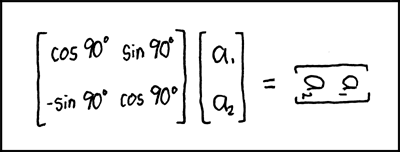
\includegraphics{matrix_transform.png}

\end{center}
\clearpage
\tableofcontents
\clearpage
\setcounter{page}{1}
\section{Jordan}
Tipp: \enquote{Kochen mit Jordan} von Daniel Winkler\footnote{http://www.danielwinkler.de/la/jnfkochrezept.pdf}
\subsection{Jordan Normalform}
Vorgehen:
\begin{itemize}
	\item Charakteristisches Polynom berechnen (Eigenwerte)
	\begin{itemize}
		\item Anzahl der Eigenwerte = Anzahl der Jordanblöcke
		\item Algebraische VVK = Größe des Jordanblocks des Eigenwertes
		\item Geometrische VVK = Anzahl der Jordankästchen im Block
	\end{itemize}
	\item Wenn mehrere Möglichkeiten Kästchen zu bilden:
	\begin{itemize}
		\item Index des Hauptraumes herausfinden
		\item Matrix hochnehmen bis sie sich nicht mehr ändert (oft Nullmatrix)
		\item Index = größtes Jordankästchen im Block
	\end{itemize}
	\item Per Konvention: größte Jordanblöcke und -kästchen zuerst
	\item Minimalpolynom $m_p$: Wie Charakteristisches Polynom, Potenzen aber wie das größte Jordankästchen zum Eigenwert.
\end{itemize}
\subsubsection*{Lösen von Allgemeinen Aufgaben}
Zum lösen von allgemeinen Aufgaben ohne konkret gegebene Matrix hilft:
\begin{itemize}
	\item Größe der Matrix = Größe der JNF (= Dimension???)
	\item Spur der Matrix = Spur der JNF
	\item Wenn gegeben: Größe, Eigenwerte, Spur: Jordan\textbf{blöcke} ausrechenbar
	\item Wenn Hauptraumgleichung $\neq 0$, dann Jordan\textbf{kästchen} größer als Potenz\\
		bsp: $(A-I_i)^2 \neq 0 \Rightarrow$ Jordankästchen vom EW $i$  $\geq 3$ (falls Jordanblock $>2$ )
\end{itemize}
\subsection{Bestimmung der Basiswechselmatrix S}
Hauptraum: Kleinste Zahl $p$, für die gilt: $Kern(A-\lambda I)^p = Kern(A-\lambda I)^{p+1}$\\
\begin{itemize}
	\item Nehme Basisvektoren aus $Kern(A-\lambda I)^p$, welche nicht in  $Kern(A-\lambda I)^{p-1}$ enthalten sind $\Rightarrow v_1, v_2, ...$
	\item Die Geordnete Basis ist definiert durch: \\
		$v_1, (A-\lambda I)\cdot v_1, (A-\lambda I)^2\cdot v_1,\; \hdots\; , v_2, (A-\lambda I)\cdot v_2, (A-\lambda I)^2\cdot v_2,\; \hdots$\\
		(jeweils bis $(A-\lambda I)^{p-1}$)
	\item Falls Jordankästchen des EW der Größe $p-1$ existiert, Schritte wiederholen für $p \rightarrow p-1$
	\item Diese Schritte wür alle EW wiederholen
	\item Falls noch nicht alle Vektoren für die Basis vorhanden: Vektoren aus $Kern(A-\lambda I)$ hinzufügen, welche linear unabhängig sind
	
\end{itemize}
\section{Isometrienormalform}
\begin{itemize}
	\item Hilfsmatrix $H = A+A^T$ bestimmen
	\item Eigenwerte von $H$ bestimmen
	\item Isometrienormalform erstellen
	\begin{itemize}
	
		\item Algebraische VVK des Eigenwerts $2$ ist die Anzahl der $1$ auf der Hauptdiagonale
		\item Algebraische VVK des Eigenwerts $-2$ ist die Anzahl der $-1$ auf der Hauptdiagonale
		\item Die anderen Eigenwerte müssen $\in (-2,2)$ liegen
		\item Für die anderen Eigenwerte gilt weiterhin das \\ 
			Drehkästchen: $\begin{pmatrix}
			\dfrac{\lambda}{2} & -\sqrt{1-(\dfrac{\lambda}{2})^2}\\
			\sqrt{1-(\dfrac{\lambda}{2})^2} & \dfrac{\lambda}{2}
			\end{pmatrix}$
	\end{itemize}
\end{itemize}
\subsection*{Beispiel}
$CP(H) = (2-\lambda)^2(-2-\lambda)^2(0-\lambda)$ \\
$\Rightarrow D_\lambda = 
\begin{pmatrix}
1&&&&&\\
&1&&&&\\
&&-1&&&\\
&&&-1&&\\
&&&&0&-1\\
&&&&1&0
\end{pmatrix}
$ (Leere Felder sind $0$)
\subsection{Tipps}
Hilfreich, bei allgemeinen Aufgaben ohne konkret gegebene Matrix
\begin{itemize}
	\item Können Eigenwerte $1$ und $-1$ vorkommen?
	\item Determinante und Spur von der Matrix und der Isometrienormalform sind identisch
	\item Beim $\mathbb{R}^3$ gilt: (siehe nächstes Kapitel)
	\begin{itemize}
		\item Ein Eintrag mit 1 (entspricht der Drehachse)
		\item Ein Drehkästchen
	\end{itemize}
\end{itemize}
\subsection{Basisswechselmatrix}
\begin{itemize}
	\item Für $H$ die Eigenräume von $\pm 2$ berechnen und in Orthonormalbasis umwandeln (ablesbar, oder Gram-Schmidt-Verfahren) \\
	$\Rightarrow$ Man erhält die ersten Spalten
	\item Für die anderen Eigenwerte Eigenräume ausrechnen.\\
	Ein $v$ wählen und mit $\tilde{A}v$ orthonalisieren und Normalisieren (Gram-Schmidt) \\
	Falls Eigenraum Dimension $2$ hat, mit nächstem Eigenraum fortfahren
\end{itemize}
\subsection{Gram-Schmidt Verfahren zur Orthonormalbasis}
\begin{itemize}
	\item gegeben: Basis $(b_1, \hdots ,b_n)$ \\
		gesucht: Orthonormalbasis $(c_1, \hdots ,c_n)$
	\item Wähle einen Vektor aus der Basis und normiere ihn $\Rightarrow c_1$
	\item $c_2' = b_2 - \langle b_2 \cdot c_1 \rangle \cdot c_1$ \\
		$c_2 = \frac{1}{|c_2'|}\cdot c_2'$ ($c_2'$ Normieren)
	\item $c_3' = b_3 - \langle b_3 \cdot c_2 \rangle \cdot c_2 - \langle b_3 \cdot c_1 \rangle \cdot c_1$ \\
	$c_3 = \frac{1}{|c_3'|}\cdot c_3'$ ($c_3'$ Normieren)
	\item und so weiter
\end{itemize}

\section{Drehachse und -winkel}
\begin{itemize}

\item Drehebene: $[x-\Phi(x),y-\Phi(y)]$ 
\item Drehachse: Finde einen Vektor $v$, für den gilt:
\begin{itemize}
	\item $\langle x-\Phi(x),v\rangle=0$
	\item $\langle y-\Phi(y),v\rangle=0$
\end{itemize}
\item Drehwinkel: Finde einen Vektor $u$, für den gilt:
\begin{itemize}
	\item Orthgonal zur Drehachse
	\item Bild kann berechnet werden
	\item $\Rightarrow u$ ist Linearkombination aus $x,y,v$
\end{itemize}
\end{itemize}
\subsection{Vorgehen Drehwinkel}
\begin{itemize}
	\item Wähle ein $u \in $ Drehebene
	\item Löse folgendes LGS: $u=ax+by+cv$
	\item Berechne $\Phi(u) = a \cdot \Phi(x) + b \cdot \Phi(y)+ c \cdot \Phi(v)$ \\
		(Da $v$ Drehachse, gilt $\Phi(v) = v$)
	\item Berechne Winkel zwischen $\Phi(u)$ und $u$:\\
		$\cos \alpha = \frac{\langle x,y\rangle}{||x|| \cdot ||y||}$
\end{itemize}
\subsection{Isometrienormalform aus dem Drehwinkel im $\mathbb{R}^3\times\mathbb{R}^3$}
Die Isometrienormalform im $\mathbb{R}^3$ besteht immer aus:
\begin{itemize}
	\item Ein Eintrag mit 1
	\item Ein Drehkästchen
	\item also: $\begin{pmatrix}
1&0&0 \\
0&D_\lambda&\\
0&&
\end{pmatrix}$
	\item $D_\varphi = \begin{pmatrix}
\cos \varphi & -\sin \varphi \\
\sin \varphi & \cos \varphi
\end{pmatrix}$
	\item $\sin = \sqrt{1-\cos^2}$
\end{itemize}
Merke auch die Matrix $D_\lambda$ unter dem Punkt Isometrienormalform
\section{Bestimmung von Basiswechselmatrix zu Isometrie}
\begin{itemize}
	\item Bestimme Eigenräume zu Eigenwerten von $H=A+A^T$
	\item Bestimme insgesamt ONB aus Eigenräumen
	\item Vorletzter Basisvektor $b_{n-1}$ nehmen \\
		$A\cdot b_{n-1}$ berechnen und als Linearkombination von $b_{n} \text{ und } b_{n-1}$ darstellen
	\begin{itemize}
		\item Falls $b_{n-1} = \hdots b_{n-1} + \hdots b_{n}$, be happy
		\item Falls $b_{n-1} = \hdots b_{n-1} - \hdots b_{n}$, mit $-1$ Multiplizieren
	\end{itemize}
	\item $b_1, \hdots b_n$ sind die Spalten der Basiswechselmatrix $S$
\end{itemize}
\section{Skalarproduktbeweis}
\begin{itemize}
	\item Symmetrie Zeigen: $\langle x,y \rangle = \langle y,x \rangle$
	\item Bilinearform Zeigen:
	\begin{itemize}
		\item $\langle A_1+A_2,B\rangle = \langle A_1,B\rangle + \langle A_2,B\rangle$
		\item $\langle c \cdot A,B \rangle = c \cdot \langle A,B\rangle$
	\end{itemize}
	\item Positive Definitheit zeigen
	\begin{itemize}

		\item $\langle x,x \rangle > 0 $ (für $x \neq 0$)
		\item $\langle x,x \rangle = 0 $ (nur für $x = 0$)
	\end{itemize}
\end{itemize}
\section{Orthogonales Komplement}
\begin{itemize}
	\item Vektoren von $U$ horizontal in eine Matrix Schreiben
	\item Kern der Matrix ausrechnen (Gauß und -1-Trick)
	\item Kern = Basis von $U^\perp$
\end{itemize}
\section{Orthogonale Projektion $\pi_U(v)$}
\begin{itemize}
	\item Bestimme ONB von $U$: $b_1, \hdots b_n$
	\item $\pi_U(v) = \langle v,b_1\rangle \cdot b_1 + \cdots + \langle v,b_n\rangle \cdot b_n$
\end{itemize}
Abstand $d(v,U) = ||\pi_U(v)||$
\section{Abstand von Untervetorräumen}
\begin{itemize}
	\item 
\end{itemize}
\section{Formeln}
\begin{itemize}
	\item Winkel zwischen 2 Vektoren $\cos \alpha = \frac{\langle x,y \rangle}{||x|| \cdot ||y||}$
	\item 2 Vektoren orthogonal, wenn $\langle x,y \rangle = 0$
\end{itemize}
\end{document}
